%----------------------------------------------------------------------------------------
%   Доорх хэсгийг өөрчлөх шаардлагагүй
%----------------------------------------------------------------------------------------
%!TEX TS-program = xelatex
%!TEX encoding = UTF-8 Unicode
\documentclass[12pt,A4]{report}

\usepackage{fontspec,xltxtra,xunicode}
\setmainfont[Ligatures=TeX]{Times New Roman}
\setsansfont{Arial}

% \usepackage[utf8x]{inputenc}
% \usepackage[mongolian]{babel}
%\usepackage{natbib}
\usepackage{geometry}
%\usepackage{fancyheadings} fancyheadings is obsolete: replaced by fancyhdr. JL
\usepackage{fancyhdr}
\usepackage{float}
\usepackage{afterpage}
\usepackage{graphicx}
\usepackage{amsmath,amssymb,amsbsy}
\usepackage{dcolumn,array}
\usepackage{tocloft}
\usepackage{dics}
\usepackage{nomencl}
\usepackage{upgreek}
\newcommand{\argmin}{\arg\!\min}
\usepackage{mathtools}
\usepackage[hidelinks]{hyperref}

\usepackage{algorithm}
\usepackage{algpseudocode}

\usepackage{listings}
\DeclarePairedDelimiter\abs{\lvert}{\rvert}%
\makeatletter
\usepackage{caption}
\captionsetup[table]{belowskip=0.5pt}
\usepackage{subfiles}

\usepackage{listings}
\renewcommand{\lstlistingname}{Код}
\renewcommand{\lstlistlistingname}{\lstlistingname ын жагсаалт}

\usepackage{color}
\definecolor{codegreen}{rgb}{0,0.6,0}
\definecolor{codegray}{rgb}{0.5,0.5,0.5}
\definecolor{codepurple}{rgb}{0.58,0,0.82}
\definecolor{backcolour}{rgb}{0.99,0.99,0.99}

\lstdefinestyle{mystyle}{
    basicstyle=\ttfamily\small,
    backgroundcolor=\color{backcolour},
    commentstyle=\color{codegreen},
    keywordstyle=\color{magenta},
    numberstyle=\tiny\color{codegray},
    stringstyle=\color{codepurple},
    %basicstyle=\footnotesize,
    breakatwhitespace=false,
    breaklines=true,
    captionpos=b,
    keepspaces=false,
    numbers=left,
    numbersep=10pt,
    showspaces=false,
    showstringspaces=true,
    showtabs=false,
    tabsize=2
}

\lstset{style=mystyle, label=DescriptiveLabel}

\let\oldabs\abs
\def\abs{\@ifstar{\oldabs}{\oldabs*}}
\makenomenclature
\begin{document}


%----------------------------------------------------------------------------------------
%   Өөрийн мэдээллээ оруулах хэсэг
%----------------------------------------------------------------------------------------

% Дипломийн ажлын сэдэв
\title{Веб аппликейшн хөгжүүлэлт}
% Дипломын ажлын англи нэр
\titleEng{Web application development}
% Өөрийн овог нэрийг бүтнээр нь бичнэ
\author{Энхбаярын Жавхлан}
% Өөрийн овгийн эхний үсэг нэрээ бичнэ
\authorShort{Э.Жавхлан}
% Удирдагчийн зэрэг цол овгийн эхний үсэг нэр
\supervisor{Т.Билгүүн}
% Хамтарсан удирдагчийн зэрэг цол овгийн эхний үсэг нэр
\cosupervisor{Д.Цолмон}

% СиСи дугаар
\sisiId{20B1NUM0649}
% Их сургуулийн нэр
\university{МОНГОЛ УЛСЫН ИХ СУРГУУЛЬ}
% Бүрэлдэхүүн сургуулийн нэр
\faculty{МЭДЭЭЛЛИЙН ТЕХНОЛОГИ, ЭЛЕКТРОНИКИЙН СУРГУУЛЬ}
% Тэнхимийн нэр
\department{МЭДЭЭЛЭЛ, КОМПЬЮТЕРИЙН УХААНЫ ТЭНХИМ}
% Зэргийн нэр
\degreeName{Үйлдвэрийн дадлагын тайлан}
% Суралцаж буй хөтөлбөрийн нэр
\programeName{Програм хангамж(D061302)}
% Хэвлэгдсэн газар
\cityName{Улаанбаатар}
% Хэвлэгдсэн огноо
\gradyear{2024 оны 02 сар}


%----------------------------------------------------------------------------------------
%   Доорх хэсгийг өөрчлөх шаардлагагүй
%----------------------------------------------------------------------------------------
%----------------------Нүүр хуудастай хамаатай зүйлс----------------------------
\pagenumbering{roman}
\maketitle

\doublespace

% Decleration
\begin{huge}
\textbf{Зохиогчийн баталгаа}
\end{huge} \\ \ \\
\doublespace
Миний бие \@author \ \@degreeName г\ хийж гүйцэтгэсэн болохыг зарлаж дараах зүйлсийг баталж байна:
\begin{itemize}
\item Бусдын хийсэн ажлаас хуулбарлаагүй, ашигласан бол ишлэл, зүүлт хийсэн.
\item Ажлыг би өөрөө (хамтарч) хийсэн ба миний хийсэн ажил, үзүүлсэн дэмжлэгийг тайлангийн ажилд тодорхой тусгасан.
\item Ажилд тусалсан бүх эх сурвалжид талархаж байна.
\end{itemize}
\

Гарын үсэг: \underline{\hspace{5cm}}

Огноо: 	\ \ \underline{\hspace{3cm}}

% Гарчгийг автоматаар оруулна
\setcounter{tocdepth}{1}
\tableofcontents

% Зургийн жагсаалтыг автоматаар оруулна
\listoffigures

% Хүснэгтийн жагсаалтыг автоматаар оруулна
\listoftables

% Кодын жагсаалтыг автоматаар оруулна
\lstlistoflistings

% This puts the word "Page" right justified above everything else.
\newpage
%% \addtocontents{lof}{Зураг~\hfill Хуудас \par}
\newpage
%% \addtocontents{lot}{Хүснэгт~\hfill Хуудас \par}

\renewcommand{\cftlabel}{Зураг}


\doublespace
\pagenumbering{arabic}


% Удиртгалыг оруулж ирэх ба abstract.tex файлд удиртгалаа бичнэ
\begin{abstract}
Миний бие \@author \ үйлдвэрийн дадлагын ажлыг “Зочил технологи” ХХК  компани дээр гүйцэтгэсэн. Энэхүү үйлдвэрийн дадлагын хүрээнд хичээлээс болон бие даан эзэмшсэн мэдлэг, чадвараа ашиглан бодит ажлын орчинд бүтээгдэхүүн хөгжүүлж бодит хэрэглэгчдийн гарт хүргэх процесст суралцаж React болон Bootstrap технологиуд дээр түлхүү ажилласан. Уг технологиудыг ашиглан Zochil платформын Админ вэб дээр хэрхэн  хөгжүүлэлт хийж эцсийн бүтээгдэхүүнийг гаргадаг талаар судлан хэрэгжүүлэж дадлагаа гүйцэтгэлээ.

\textbf{Зорилго:} React технологийн талаар судалж, компанийн хөгжүүлэлтийн арга барилтай танилцах.

\textbf{Зорилт:} Удирдагчийн зааварчилгааны дагуу алхам алхмаар судалгаа хийж өгсөн шаардлагын хүрээнд хэрэгжүүлэлт хийх.

\end{abstract}


%----------------------------------------------------------------------------------------
%   Дипломын үндсэн хэсэг эндээс эхэлнэ
%----------------------------------------------------------------------------------------
%\addcontentsline{toc}{part}{БҮЛГҮҮД}
% Шинэ бүлэг

\begin{table}[h]
	\caption{Дадлагын ажлын төлөвлөгөө}
	\begin{tabular}{|p{0.5cm}|p{8cm}|l|l|p{3cm}|}
	\hline
	\textbf{№} & \textbf{Гүйцэтгэх ажил} & \textbf{Хугацаа} & \textbf{Биелэлт} & \textbf{Дадлагын удирдагчийн үнэлгээ} \\ \hline
	1 & Zochil платформын Админ вэб болон гар утасны Zochil IO апп-г судлах & 12/29 - 01/02 && \\ \hline
	2 & Админ вэб дээр бараа бүтээгдэхүүн болон захиалгуудын жагсаалтын responsive засах & 01/03 - 01/04 && \\ \hline
	3 & React-hook-form-г судлах & 01/03 - 01/04 && \\ \hline
	4 & React-hook-form ашиглан урсдаг зарын өгөгдлийг гараас оруулах форм үүсгэн backend-лүү дамжуулах  & 01/04 - 01/05 && \\ \hline
	5 & React-hook-form ашиглан 3 төрлийн баннер оруулах форм үүсгэн backend-лүү дамжуулах  & 01/05 - 01/07 && \\ \hline
	7 & React-hook-form ашиглан Popup сурталчилгаа оруулах форм үүсгэн backend-лүү дамжуулах  & 01/08 - 01/09 && \\ \hline
	8 & Шинээр 2 төрлийн Pricing plan хуудас үүсгэх  & 01/04 - 01/05 && \\ \hline
   9 & React-hook-form ашиглан арга хэмжээ үүсгэх форм хийж backend-лүү дамжуулах  & 01/08 - 01/09 && \\ \hline
	9 & Нэмэлт судалгааны ажил & 06/26 - 06/27 && \\ \hline

	\end{tabular}
\end{table}
\chapter{Байгууллагын танилцуулга}
\subfile{src/chapters/intro.tex}
\chapter{ИЖИЛ СИСТЕМИЙН СУДАЛГАА}
\subfile{src/chapters/similiar_system.tex}
\chapter{Системийн шаардлага}
\subfile{src/chapters/requirements.tex}
\chapter{Ашиглах технологиуд}
\subfile{src/chapters/tech.tex}
\chapter{Хэрэгжүүлэлт}
\subfile{src/chapters/body.tex}
\chapter{Нэмэлт судалгаа}
\subfile{src/chapters/JWT.tex}

%----------------------------------------------------------------------------------------
%   Дүгнэлт эндээс эхэлнэ
%----------------------------------------------------------------------------------------
\chapter{Дүгнэлт}
\section{Үр дүнгийн тайлан}
Миний бие \@author \ нэг сарын хугацаанд Зочил Технологи компанид мэргэжлийн дадлагыг амжилттай гүйцэтгэж дуусгалаа. Уг хугацаанд хичээлийн хүрээнд үзсэн онолын ойлголтуудыг практик дээр туршиж, хэрэгжүүлсэн ба хөгжүүлэлт голчилсон технологийн компанийн ерөнхий үйл ажиллагаа, баг хооронд зохицон ажиллах чадвар, хөгжүүлэлтийн шинэ арга барилуудыг амжилттай эзэмшсэн гэж дүгнэж байна.

Back-end, Front-end-ийн хамгийн орчин үеийн технологиудтай танилцаж бодит төсөл дээр ажиллаа. Мөн бие даан асуудлыг шийдэхийн тулд алхам дэс дараатай асуудлыг шийдвэрлэх мөн ашиглаж буй сан, технологийнхоо гарын авлага буюу documentation-тай илүү сайн танилцаж уг технологийнхоо цаана нь буй концептийг хялбараар ойлгох гэх мэт чадваруудыг эзэмшсэн.

Энэхүү дадлагын хугацаанд өөрийн ямар чиглэлд сонирхолтой, цаашид аль чиглэлрүү гүнзгийрэх талаараа үнэтэй туршлага цуглууллаа. Мөн жижиг стартап компанийн ажлын орчин, арга барил, болон зах зээлийн бодит амьдралыг биеэрээ мэдэрч суралцаж цаашдаа энэ замналаар нийгэмд хэрэгцээтэй шийдэл санаа хөгжүүлэх сэдлийг төрүүллээ.


%----------------------------------------------------------------------------------------
%   Дипломын номзүй, хавсралтын хэсэг эндээс эхэлнэ
%----------------------------------------------------------------------------------------

\singlespace
\addcontentsline{toc}{part}{НОМ ЗҮЙ}
\begin{thebibliography}{}
	% Ашигласан материалыг эндээс оруулна
	\bibitem{jwt}
	Introduction to JSON Web Token, \url{https://jwt.io/introduction}
	\bibitem{pillow}
	Pillow Library Documentation, \url{https://pillow.readthedocs.io/en/stable/}
	\bibitem{nuxtjs}
	Nuxtjs Documentation, \url{https://nuxt.com/docs}

\end{thebibliography}
\appendix
\addcontentsline{toc}{part}{ХАВСРАЛТ}

% Хавсралтын нэр. Хавсралт гэдэг үг агуулахгүй
\chapter{Жишээнүүд}
\begin{figure}
	\centering
	
\includegraphics[scale=2]{src/pictures/zurag1.png}
	\caption{Жишээ-1}
\end{figure}
\begin{figure}
	\centering
	
\includegraphics[scale=2]{src/pictures/zurag2.png}
	\caption{Жишээ-2}
\end{figure}
\begin{figure}
	\centering
	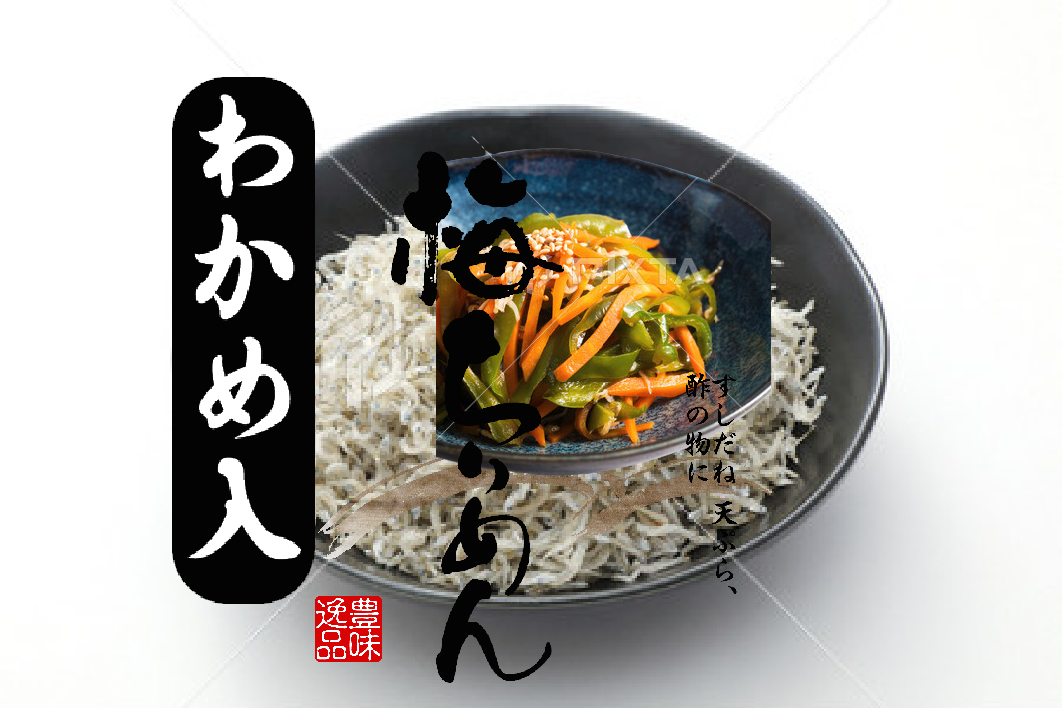
\includegraphics[scale=2]{src/pictures/zurag3.png}
	\caption{Жишээ-3}
\end{figure}

% Хавсралтын нэр. Хавсралт гэдэг үг агуулахгүй
\chapter{Кодын хэрэгжүүлэлт}
\section{Python}
\subsection{Гол script}
\lstinputlisting[language=Python, caption=Text-ээс PNG зураг үүсгэдэг script]{src/code/script.py}
\subsection{Business logic script}
\lstinputlisting[language=Python, caption=Combination үүсгэх бизнес логик код]{src/code/combination.py}
\lstinputlisting[language=Python, caption=Датабазруу КРУД хийх]{src/code/crud.py}


%----------------------------------------------------------------------------------------
%   Хавсралтууд эндээс эхэлнэ
%----------------------------------------------------------------------------------------

\end{document}
